\documentclass[12pt, titlepage]{article}

\usepackage{booktabs}
\usepackage{longtable}
\usepackage{pdflscape}
\usepackage{tabularx}
\usepackage{graphicx}
\usepackage{hyperref}
\usepackage{float}
\usepackage[round]{natbib}

\hypersetup{
    colorlinks,
    citecolor=blue,
    filecolor=black,
    linkcolor=red,
    urlcolor=blue
}

\input{../Comments}
\input{../Common}

\title{User Guide for \progname} 
\author{\authname}
\date{\today}

\begin{document}

\maketitle

\pagenumbering{roman}

\section*{Revision History}

\begin{tabularx}{\textwidth}{p{3cm}p{2cm}X}
\toprule {\bf Date} & {\bf Version} & {\bf Notes}\\
\midrule
04-11-2024 & 1.0 & Initial Version\\
27-03-2025 & 1.1 & Updates based on user feedback\\
\bottomrule
\end{tabularx}

~\newpage

\tableofcontents

\listoffigures

~\newpage

\pagenumbering{arabic}

\section{Introduction}
\subsection{Purpose}
This document serves as the user guide for RapidCare, a healthcare management system designed to streamline patient record management and medical operations. RapidCare addresses the growing shortage of family doctors in Ontario and the resulting strain on emergency rooms by reducing documentation overhead, thus allowing healthcare professionals to focus more on patient care.

\subsection{Scope}
The guide covers installation, setup, and usage of both client and server components of RapidCare. It details the process of patient documentation, voice dictation for medical notes, automated diagnosis and medicine suggestions, and healthcare network management.

\subsection{Overview}
The system consists of:
\begin{itemize}
\item Frontend ReactJS.
\item Python microservices.
\item Firebase for db and auth.
\end{itemize}

RapidCare is built to tackle documentation overhead, which currently consumes a significant portion of healthcare professionals' time. By using dictation and AI-assisted documentation, the system aims to reduce paperwork time, increase patient throughput, and improve overall care quality.

\newpage

\section{Installation}
To set up the system, follow these steps:
\subsection{Frontend Setup}
\begin{enumerate}
\item Navigate to the frontend directory.
\item Install dependencies with legacy peer dependencies support:
\begin{verbatim}
npm install --legacy-peer-deps
\end{verbatim}
\item Start the React application:
\begin{verbatim}
npm start
\end{verbatim}
\end{enumerate}
\subsection{Backend Services Setup}
For each Python service in the project:
\begin{enumerate}
\item Navigate to the service directory.
\item Install required Python packages:
\begin{verbatim}
pip install -r requirements.txt
\end{verbatim}
\item Start the service:
\begin{verbatim}
python app.py
\end{verbatim}
\end{enumerate}
\subsection{Environment Configuration}
\begin{enumerate}
\item Create a new file named \texttt{.env} in the project root directory (\texttt{src}).
\item Add the OpenAI API key configuration:
\begin{verbatim}
OPENAI_API_KEY=<your-key>
\end{verbatim}
\end{enumerate}

\newpage

\section{Usage}
\subsection{Client Interface}
\begin{figure}[H]
\centering
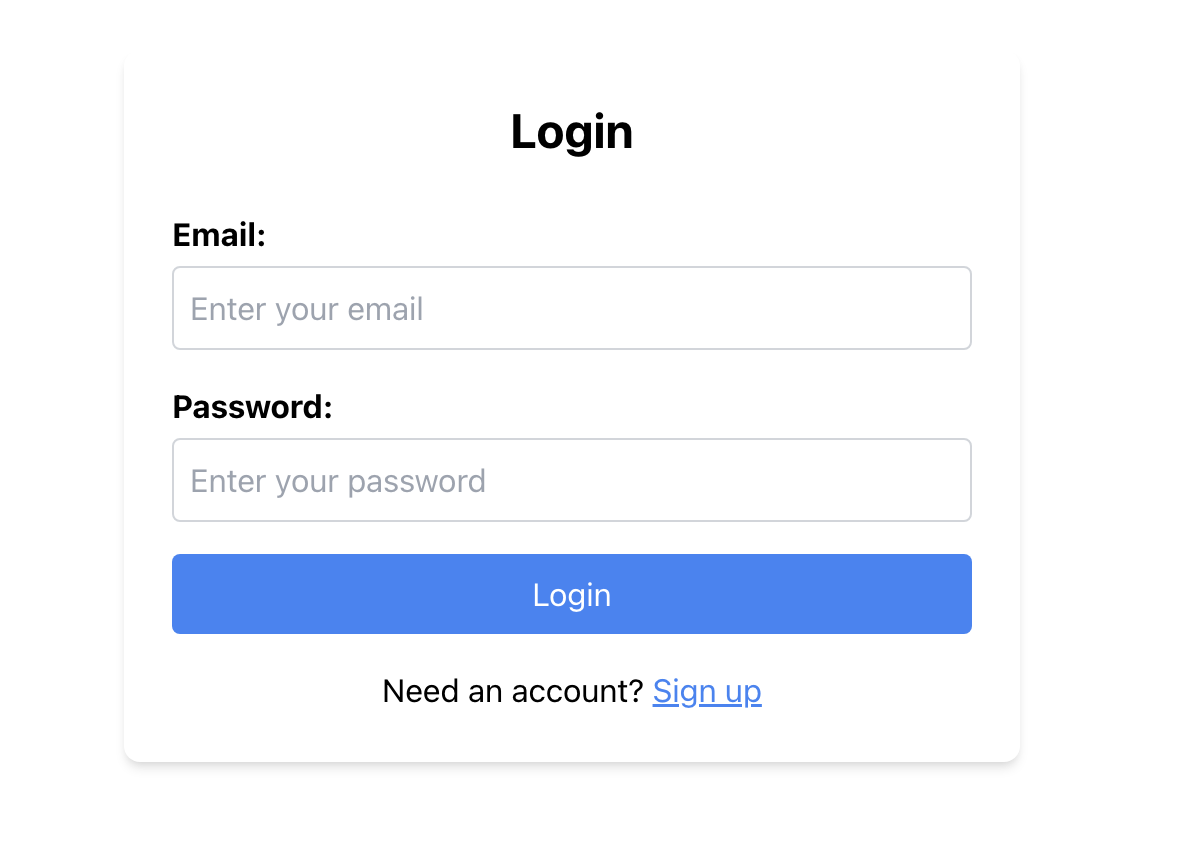
\includegraphics[width=0.8\textwidth]{login.png}
\caption{Login Screen Interface}
\label{fig:login}
\end{figure}

\subsubsection{Logging In}
\begin{itemize}
\item Enter admin/admin-provided credentials.
\item Based on credentials users are directed to their respective main page.
\item Click "Login" button.
\end{itemize}

The system will redirect you to different interfaces based on your selected role:
\begin{itemize}
\item \textbf{Admin}: Directs to the administration dashboard with system-wide management tools.
\item \textbf{Healthcare Professionals}: Directs to the hospital main page with their upcoming appointments.
\end{itemize}

\begin{figure}[H]
\centering
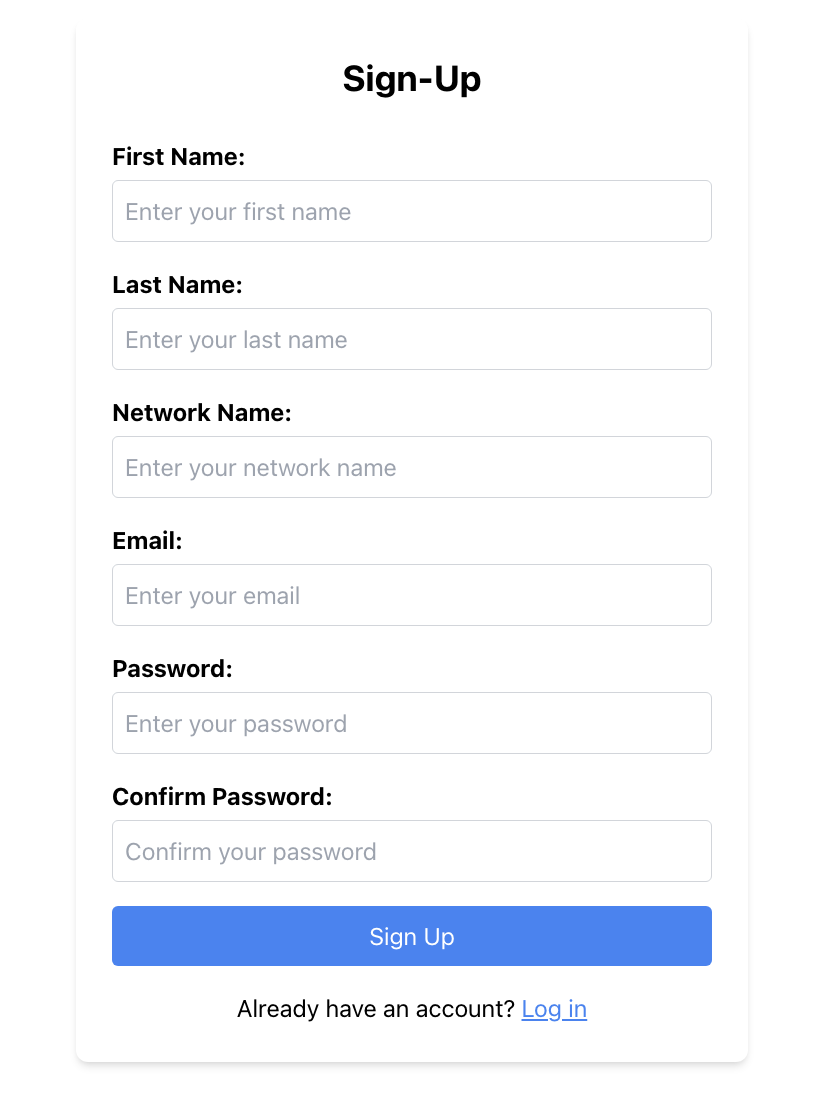
\includegraphics[width=0.8\textwidth]{signup.png}
\caption{Admin Registration Interface}
\label{fig:Registration}
\end{figure}


\subsubsection{Admin Registration}
\begin{itemize}
\item Complete the sign-up form with required admin information.
\item Include network administrator credentials.
\item Click "Sign Up" for administrative access.
\end{itemize}

\subsubsection{Administration Dashboard}
\begin{figure}[H]
\centering
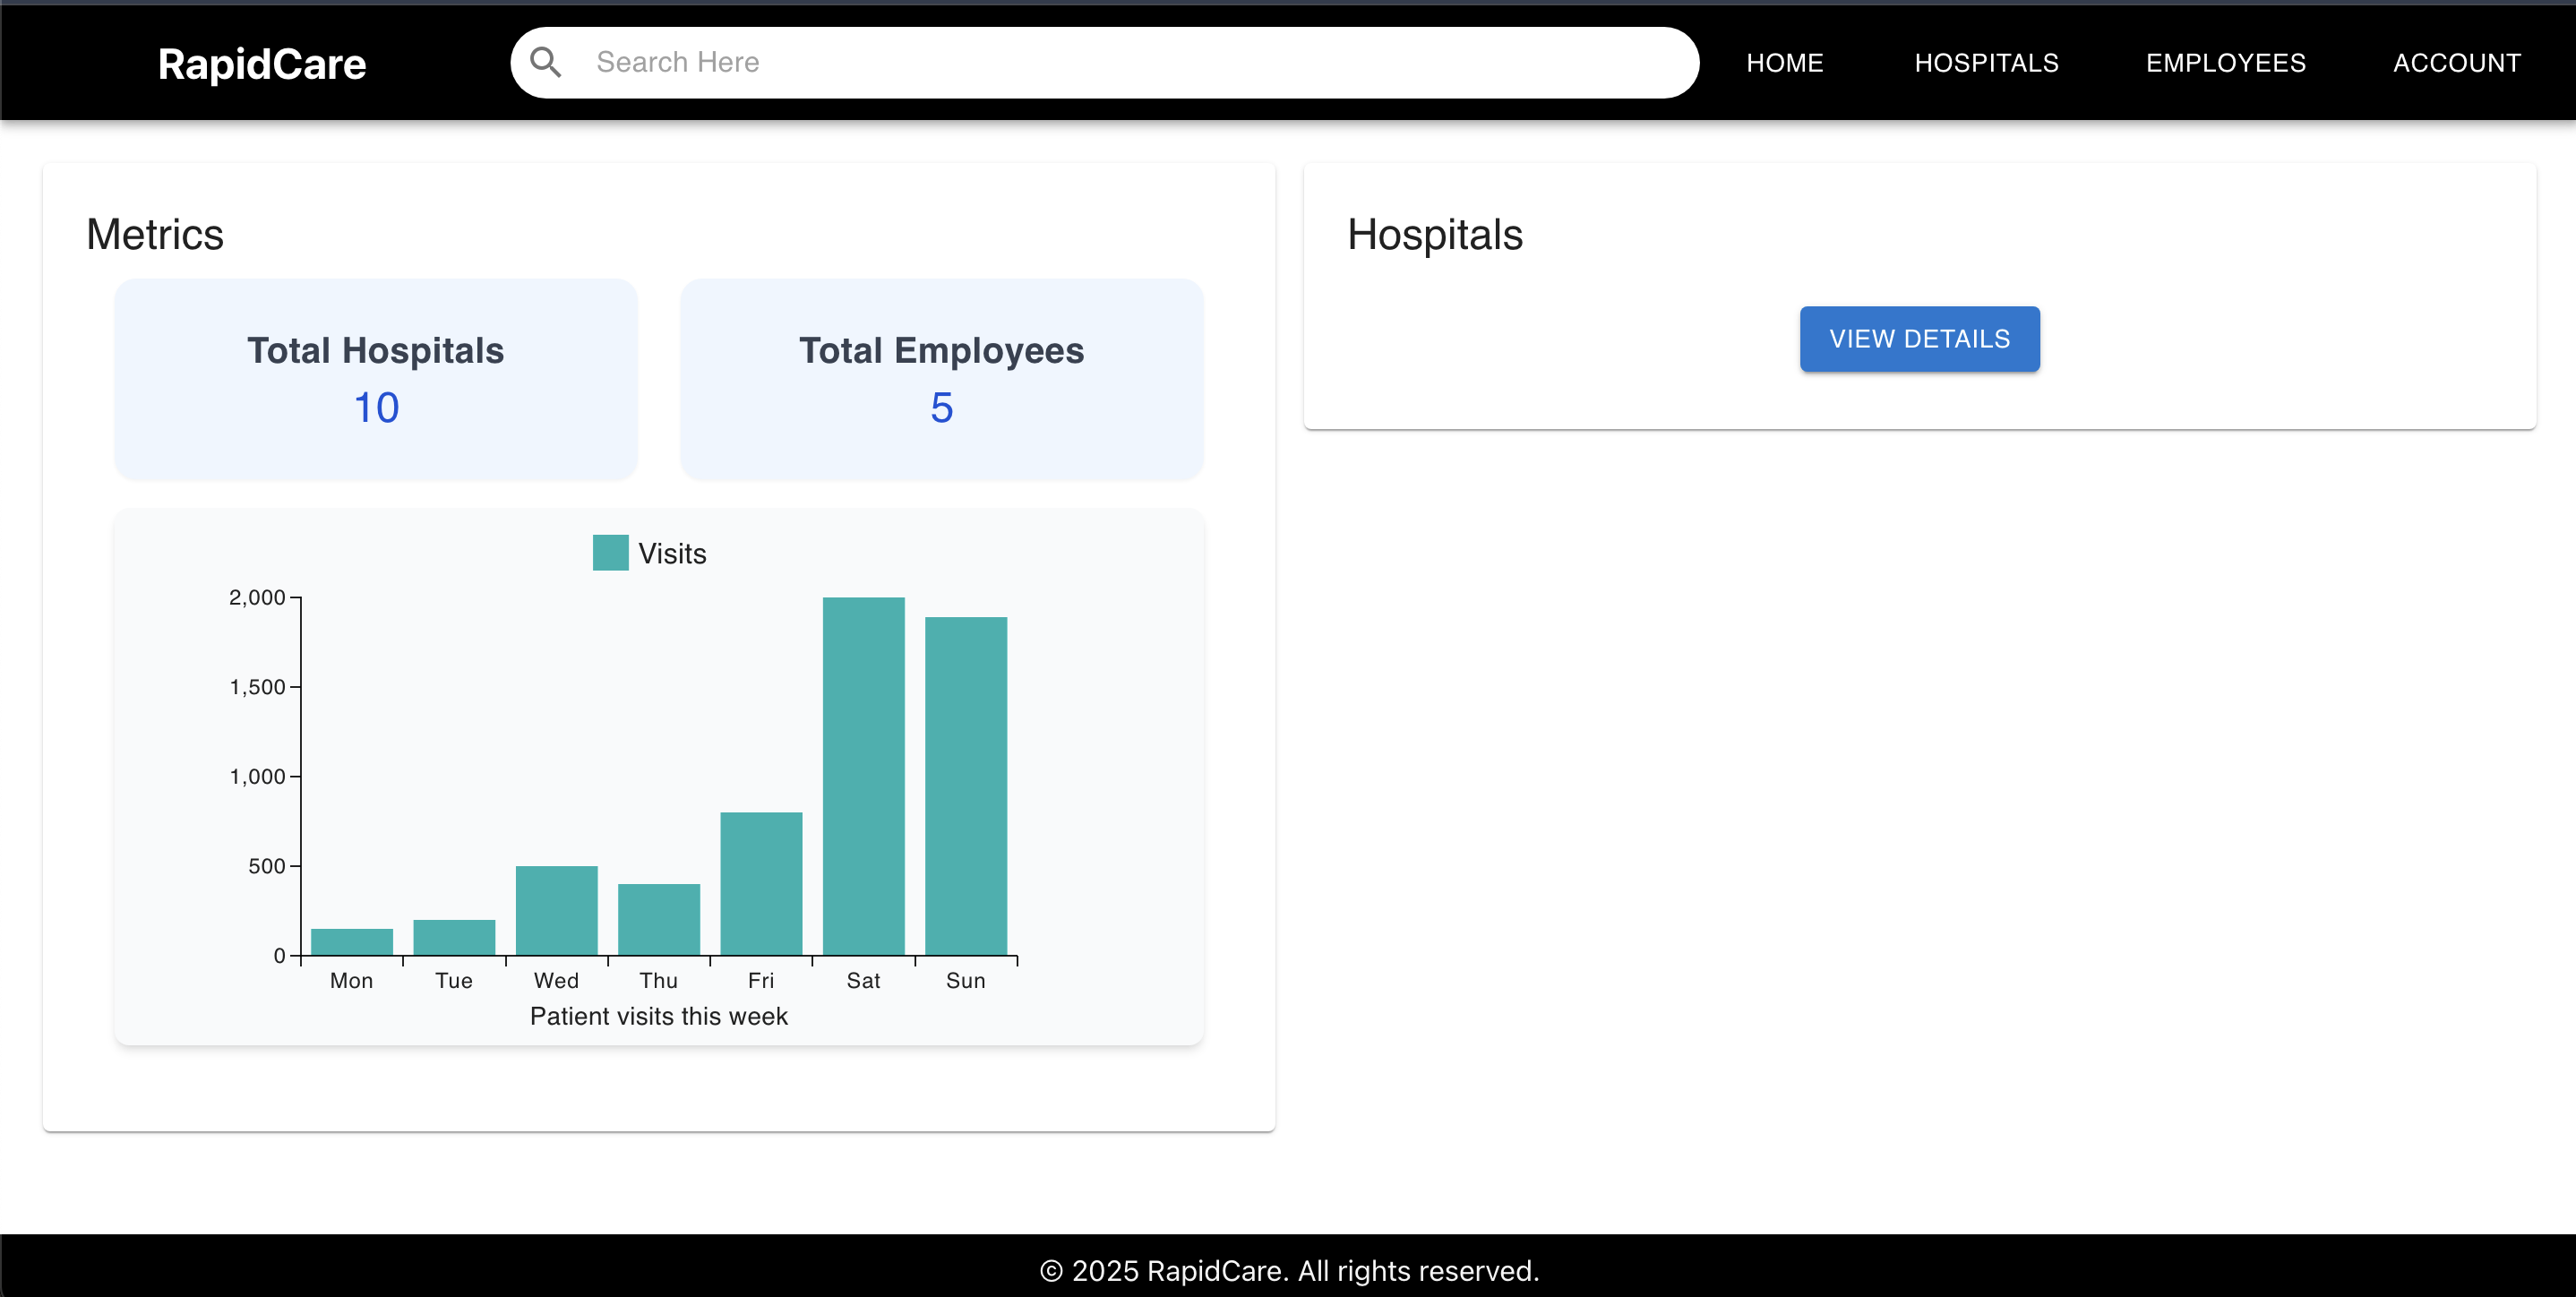
\includegraphics[width=0.8\textwidth]{admin.png}
\caption{Administrator Main Dashboard Interface}
\label{fig:admin_dashboard}
\end{figure}

The Administration Dashboard provides a comprehensive overview of network and provide network statistics, including:
\begin{itemize}
\item Account management tools.
\item Employee management tools.
\item Hospital management tools.
\end{itemize}

\subsubsection{Healthcare Professional Dashboard}
\begin{figure}[H]
\centering
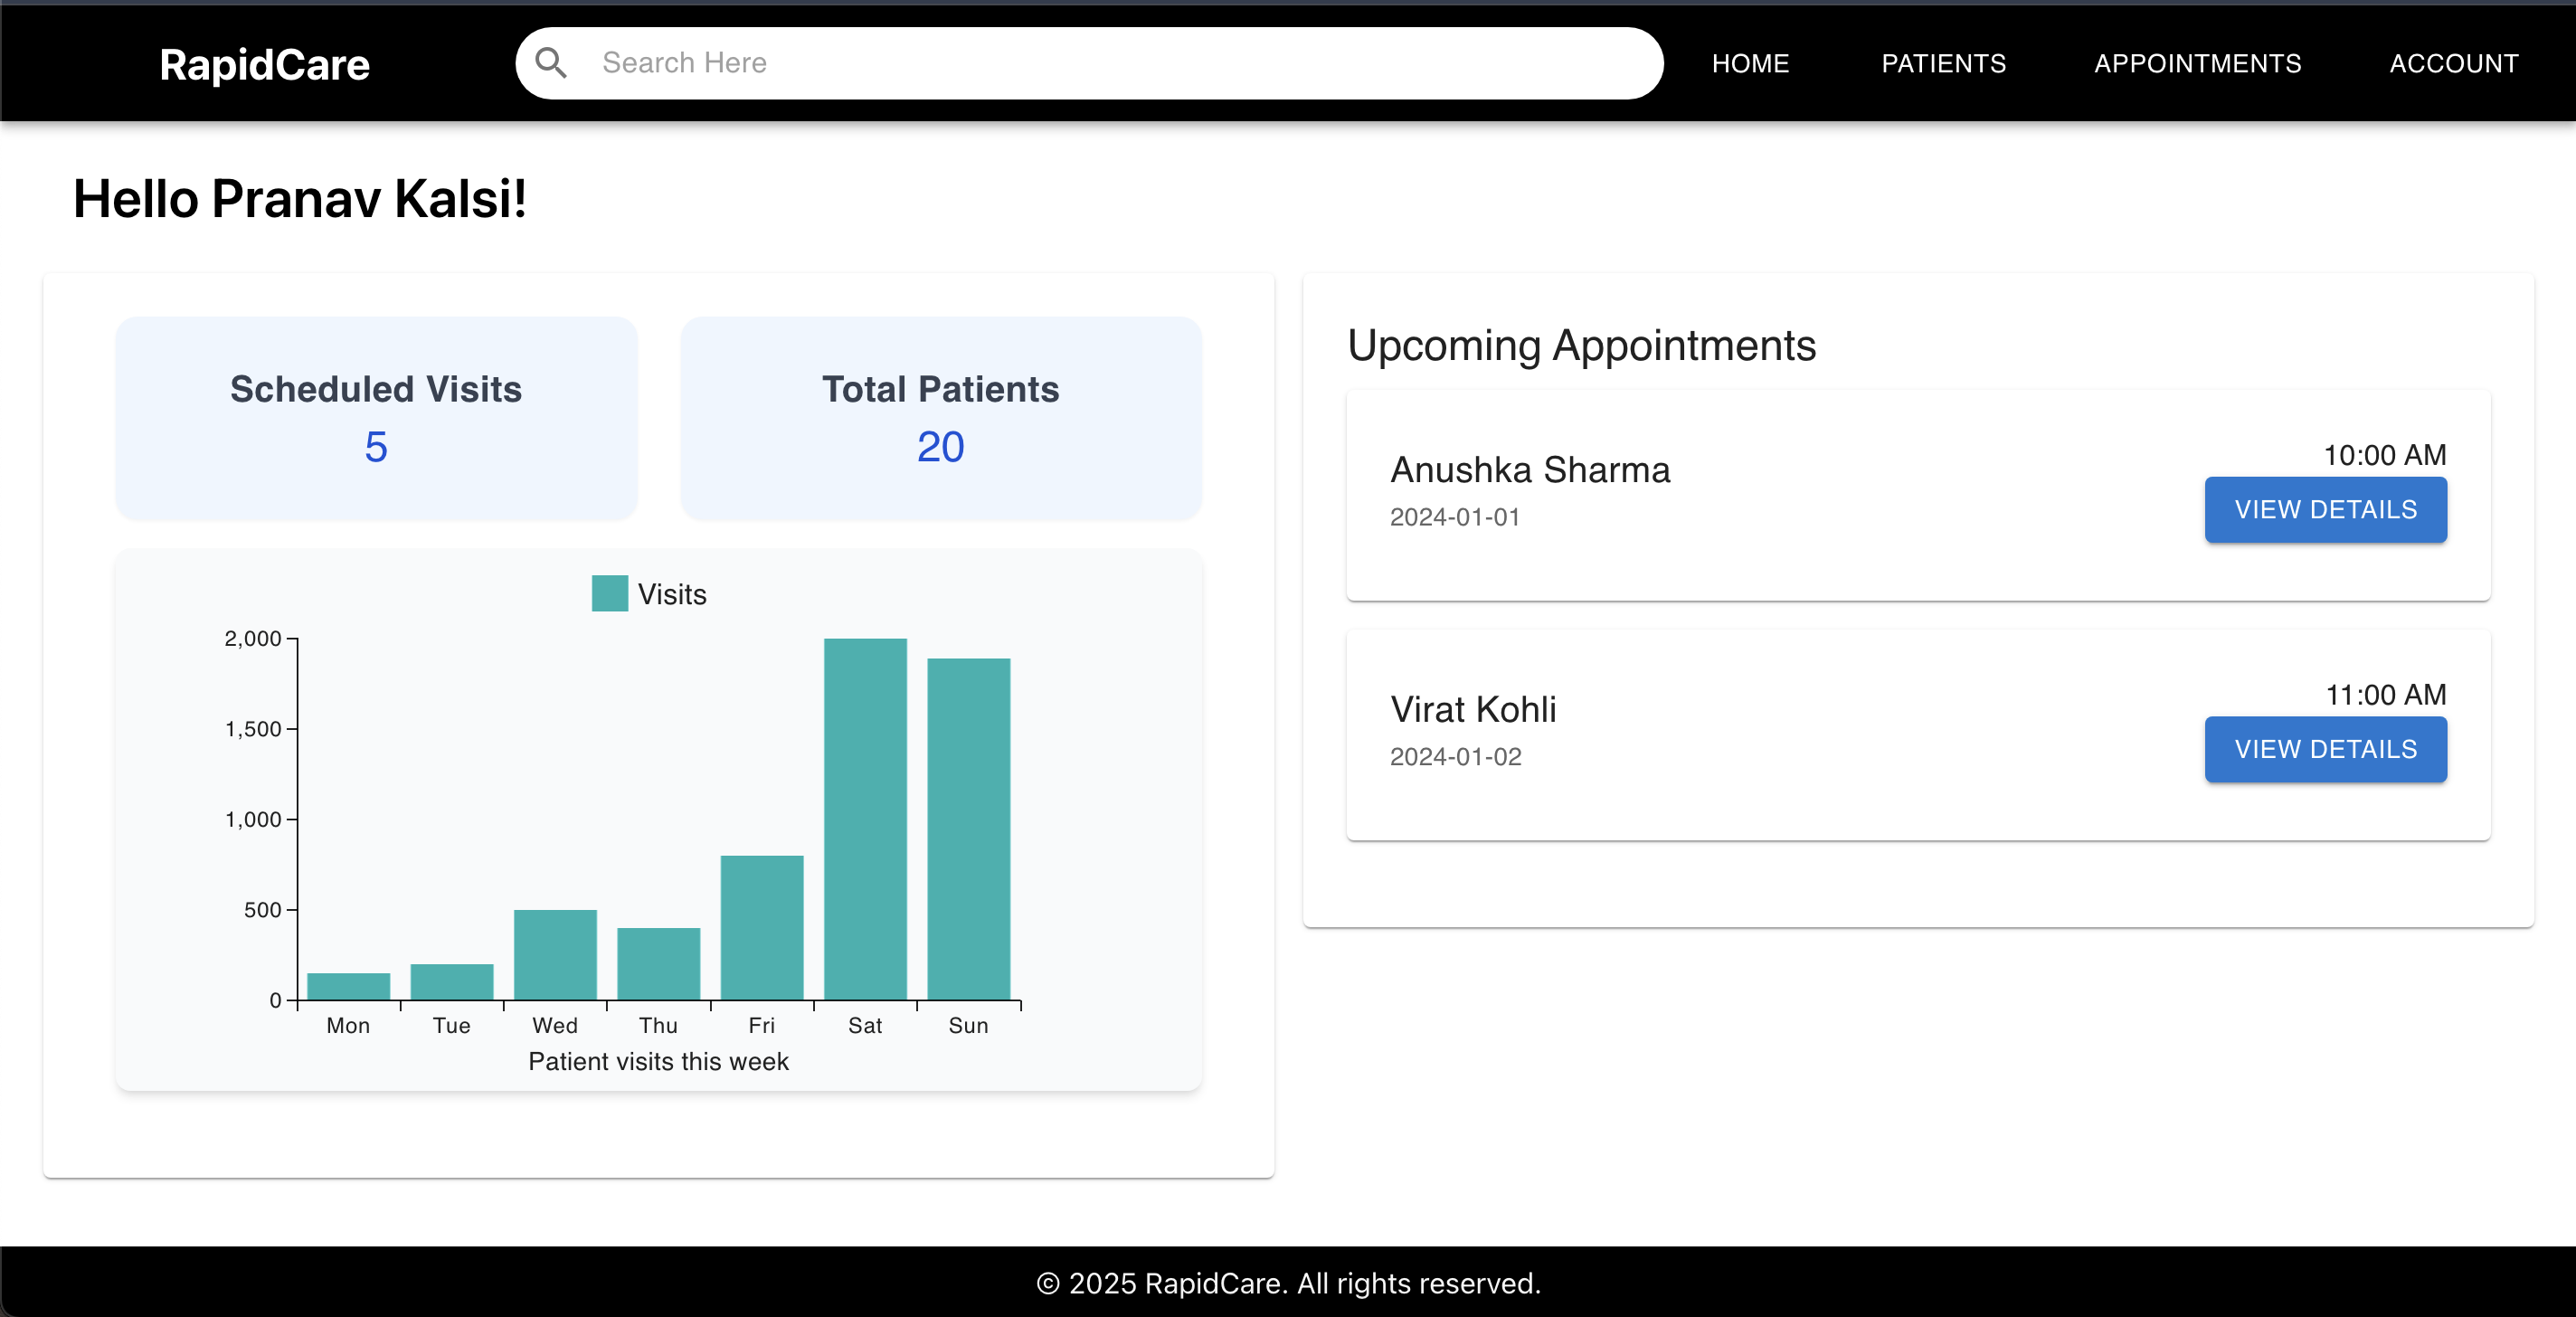
\includegraphics[width=0.8\textwidth]{healthcare.png}
\caption{Healthcare Professional Dashboard Interface}
\label{fig:healthcare_dashboard}
\end{figure}

The Healthcare Professional Dashboard provides an intuitive interface for managing patient care, including:
\begin{itemize}
\item Daily appointment schedule overview.
\item Patient visit statistics and trends.
\item Quick access to patient records.
\item Appointment management tools.
\item Account management tools.
\end{itemize}

\subsubsection{Patient Management}
\begin{longtable}{p{0.3\textwidth}p{0.6\textwidth}}
\toprule
\textbf{Action} & \textbf{Steps} \\
\midrule
Add Patient & Navigate to "Patients" tab on navbar, Click "+ Add Patient", Complete Form, "Create Patient". \\
View Records & Search for patient, Click "View Record" \\
Edit Information & Click any field, "Edit", Make Changes, "Save" \\
Remove Patient & Open Patient Records, Click "Delete Profile", Confirm Deletion \\
\bottomrule
\end{longtable}

\begin{figure}[H]
\centering
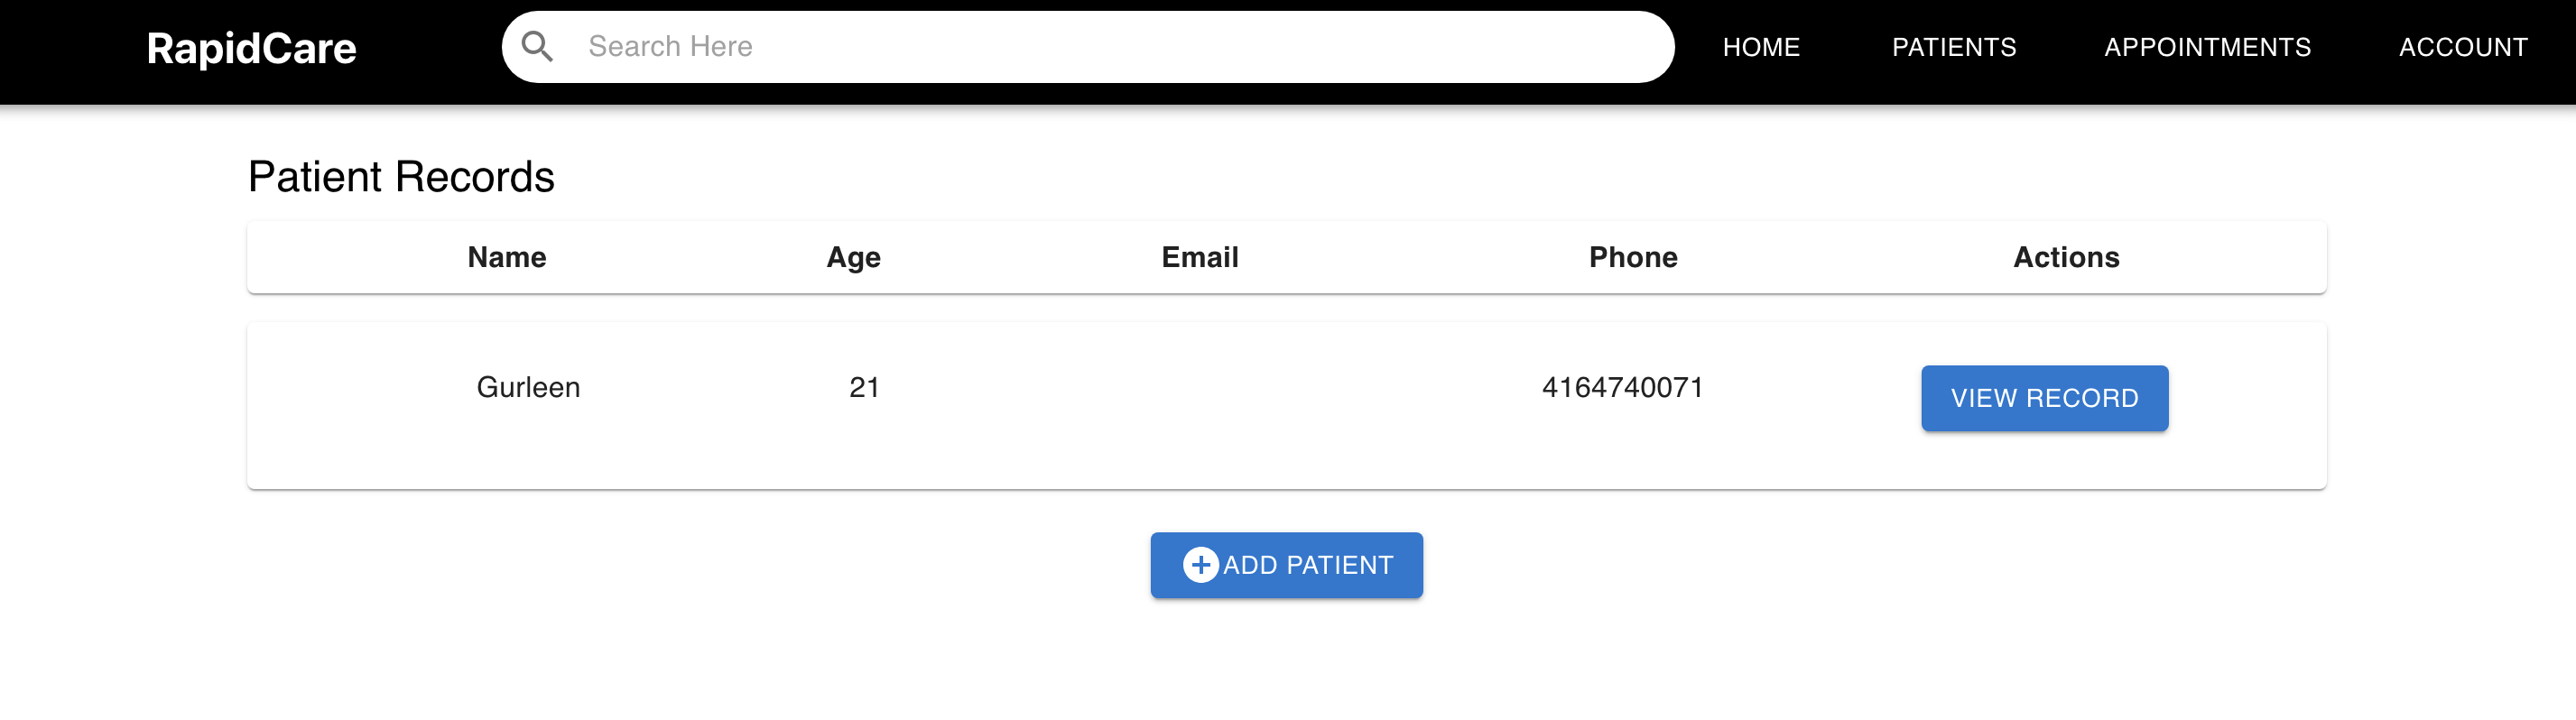
\includegraphics[width=0.9\textwidth]{patient_list.png}
\caption{Patient List}
\label{fig:Patient List}
\end{figure}

\subsubsection{Patient Record Tabs}
Once inside a patient's record, you will find several tabs on the left sidebar. Each tab serves a specific purpose in organizing and managing patient data:

\begin{figure}[H]
\centering
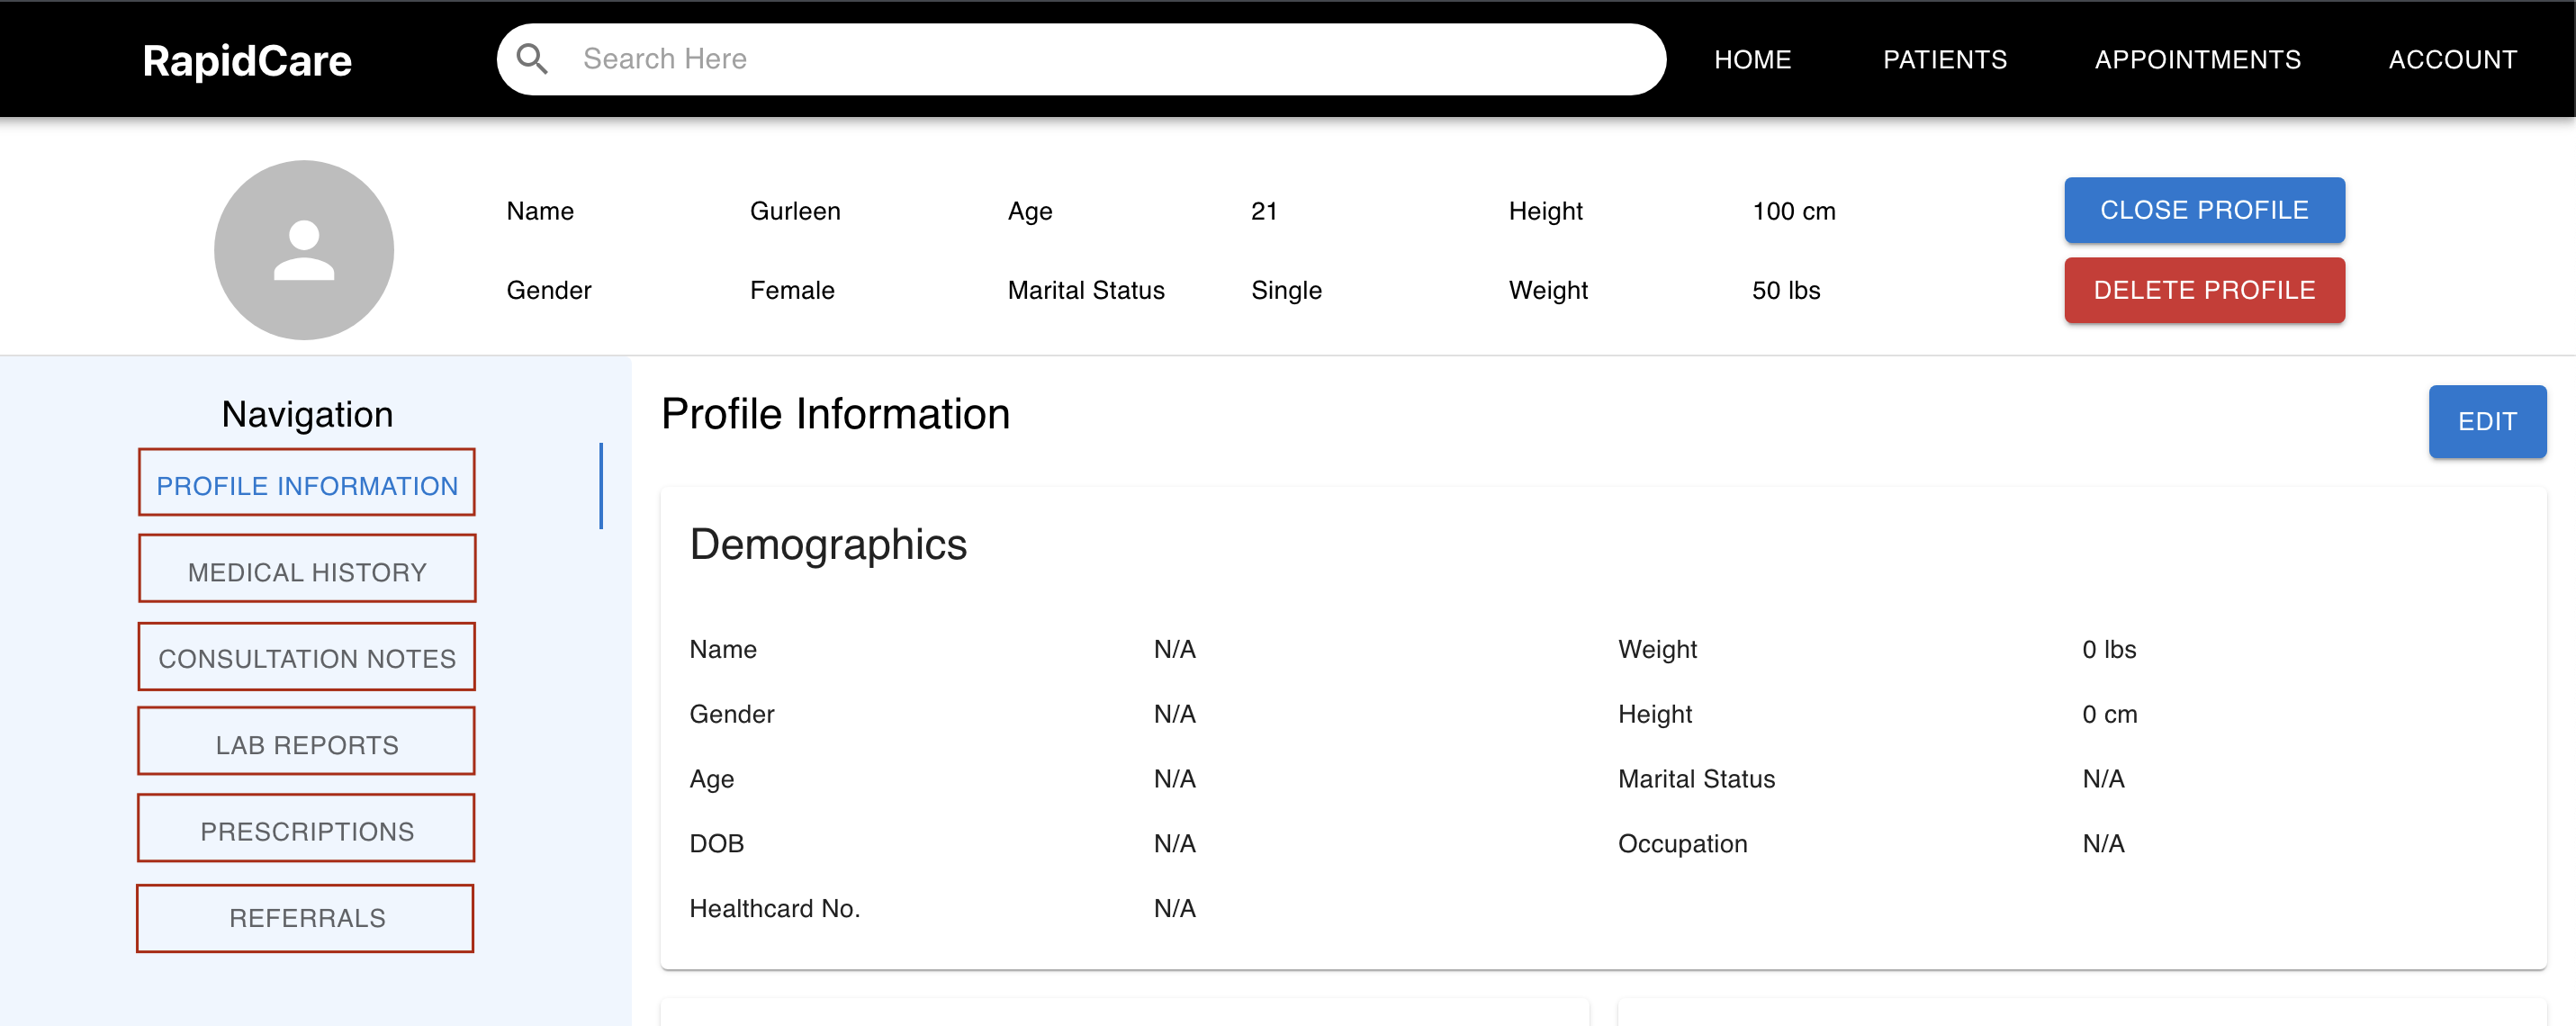
\includegraphics[width=0.9\textwidth]{patient.png}
\caption{Patient Record Tabs}
\label{fig:Patient Record Tabs}
\end{figure}
    
\begin{itemize}
    \item \textbf{Profile Information} – Displays the patient’s personal details (e.g., name, age, contact info). Click "Edit" to update any field.
    \item \textbf{Medical History} – Shows medical history, allergies, family history, and current medication. Editable via the "Edit" button.
    \item \textbf{Consultation Notes} – Used to add SOAP notes for each consultation. Click "Add New" to open the voice-enabled SOAP note interface.
    \item \textbf{Lab Reports} – Upload and view  lab documents. Use the "Add New" button to upload a new report.
    \item \textbf{Prescriptions} – Manage prescription plans. Click "Add New" to generate a medication plan for the patient.
    \item \textbf{Referrals} – Create and view referrals to other services or specialists (e.g., blood test, ultrasound). Click "Add New" and select the referral type from the drop-down.
\end{itemize}

Each tab is designed to streamline the documentation process and ensure structured, accessible patient data.


\subsection{Add a SOAP Note}

\begin{figure}[H]
\centering
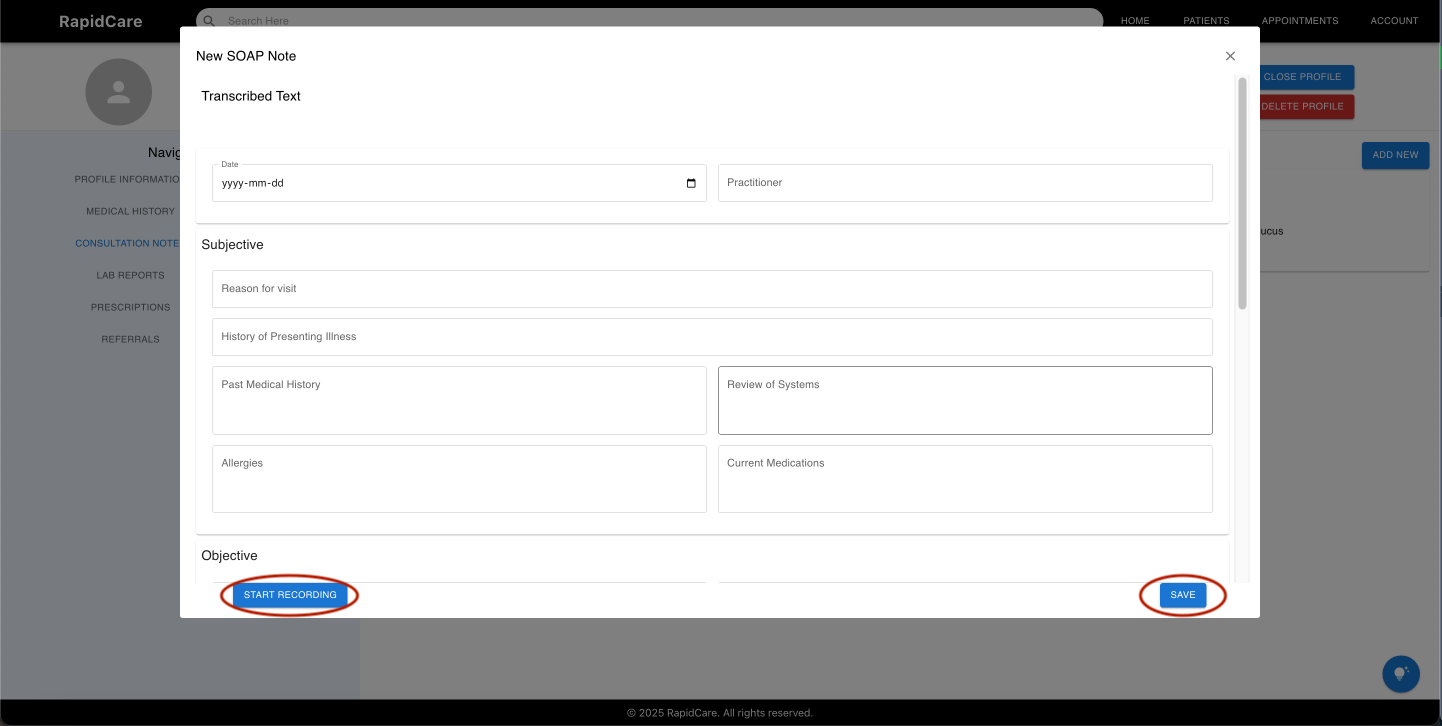
\includegraphics[width=0.8\textwidth]{vtt.png}
\caption{SOAP Note}
\label{fig:SOAP Note}
\end{figure}

RapidCare provides an end-to-end smart documentation flow under the \textbf{Consultation Notes} tab, allowing healthcare professionals to streamline SOAP note creation with AI-powered tools. Here’s how the process works:

\begin{enumerate}
    \item Log in as a healthcare professional and navigate to the \textbf{Patients} tab on the navigation bar.
    \item Search for and select the patient by clicking \textbf{View Record}.
    \item Inside the patient’s record, open the \textbf{Consultation Notes} tab from the sidebar.
    \item Click \textbf{Add New} to initiate a SOAP note. A structured pop-up will appear.
    \item Press \textbf{Start Recording} to begin capturing the patient-provider conversation.
    \item After the consultation, click \textbf{Stop Recording}. The voice-to-text microservice transcribes the recorded audio in real time.
    \item Simultaneously, the \textbf{Text Classification} microservice processes the transcription:
    \begin{itemize}
        \item It identifies symptoms, conditions, and medical terminology.
        \item Extracts key medical entities and organizes them into structured SOAP sections.
    \end{itemize}
    \item The transcribed and classified text is then passed to the \textbf{Diagnosis Suggestion Engine}, which:
    \begin{itemize}
        \item Suggests possible diagnoses based on the symptoms mentioned.
        \item Recommends a treatment plan, including medications and next steps.
    \end{itemize}
    \item The healthcare professional can review and modify any part of the classified text, diagnosis, or treatment plan.
    \item Once satisfied, click \textbf{Save} to finalize and store the SOAP note in the patient’s chart.
\end{enumerate}

This automated workflow significantly reduces manual input, improves accuracy, and accelerates clinical documentation.

\subsection{AI Assist Tool}

AI Assist feature empowers healthcare professionals to quickly gather relevant insights:

\begin{figure}[H]
\centering
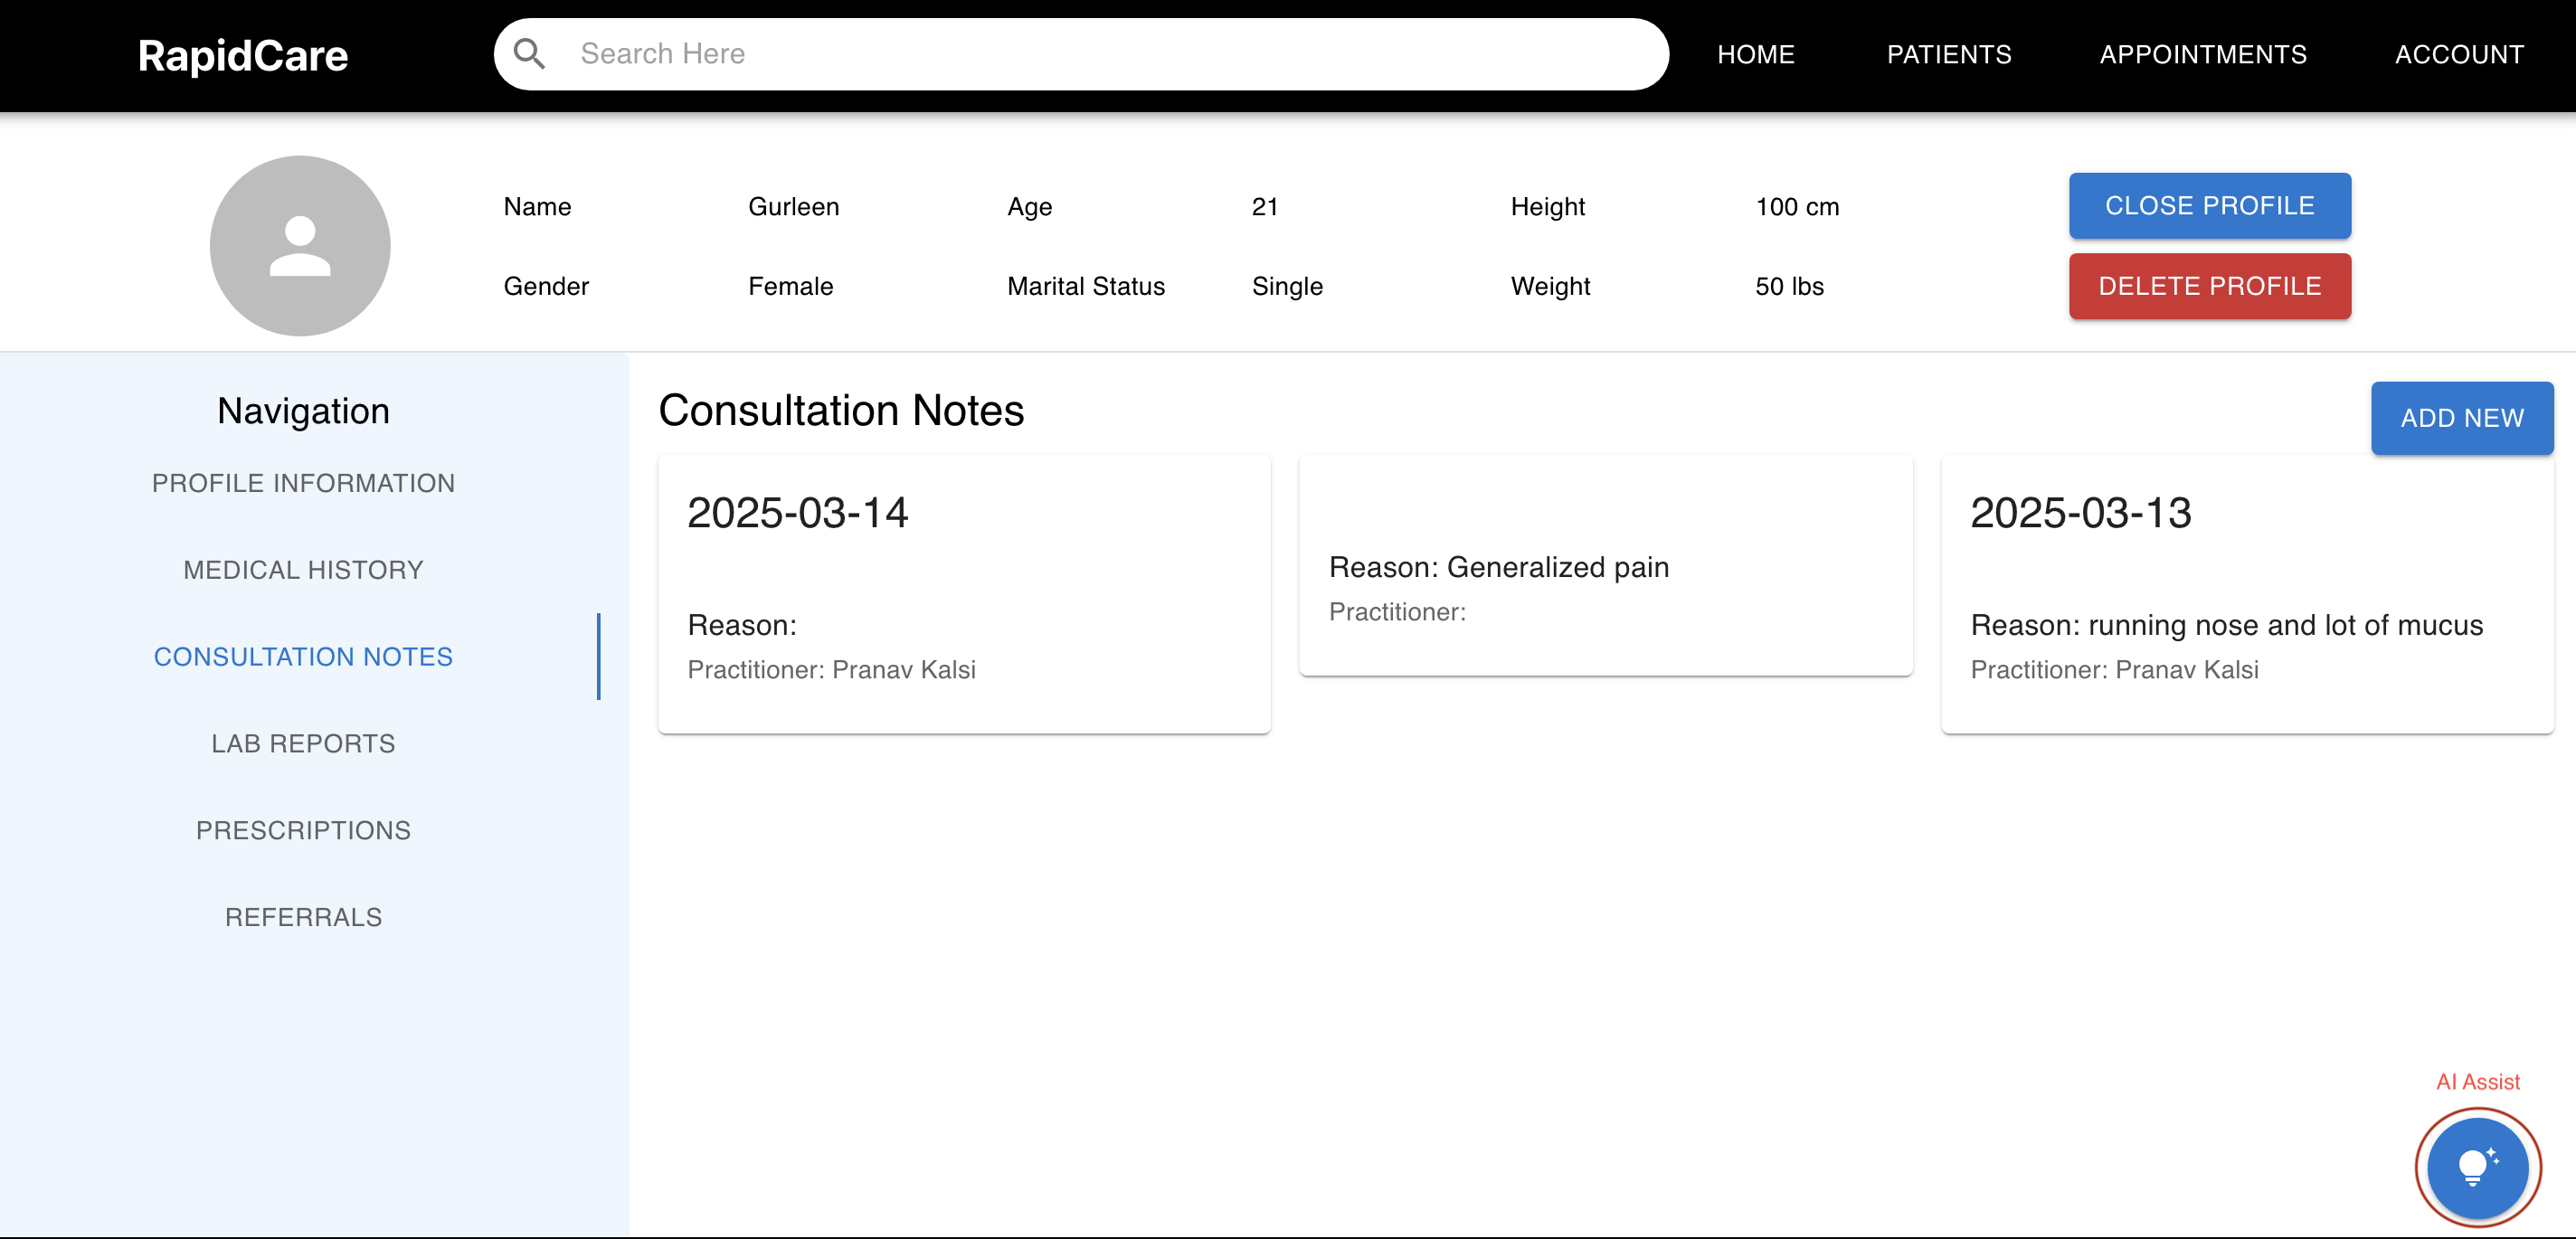
\includegraphics[width=0.9\textwidth]{AI.png}
\caption{AI Assist tool}
\label{fig:AI Assist tool}
\end{figure}

\begin{enumerate} 
\item View the patient's records to access their information. 
\item Click the AI Assist button to initiate the query. 
\item Ask any question related to the patient's data.
\item The AI will rapidly analyze the data and provide a concise response. 
\item Review the AI-generated response and incorporate them into the clinical decision-making process. 
\item Click the "X" button to exit the AI Assist panel.
\end{enumerate}

AI Assist enhances the decision-making process by surfacing relevant insights without requiring manual review of lengthy records.


\subsection{Managing Hospitals}
For hospital administrators:

\begin{figure}[H]
\centering
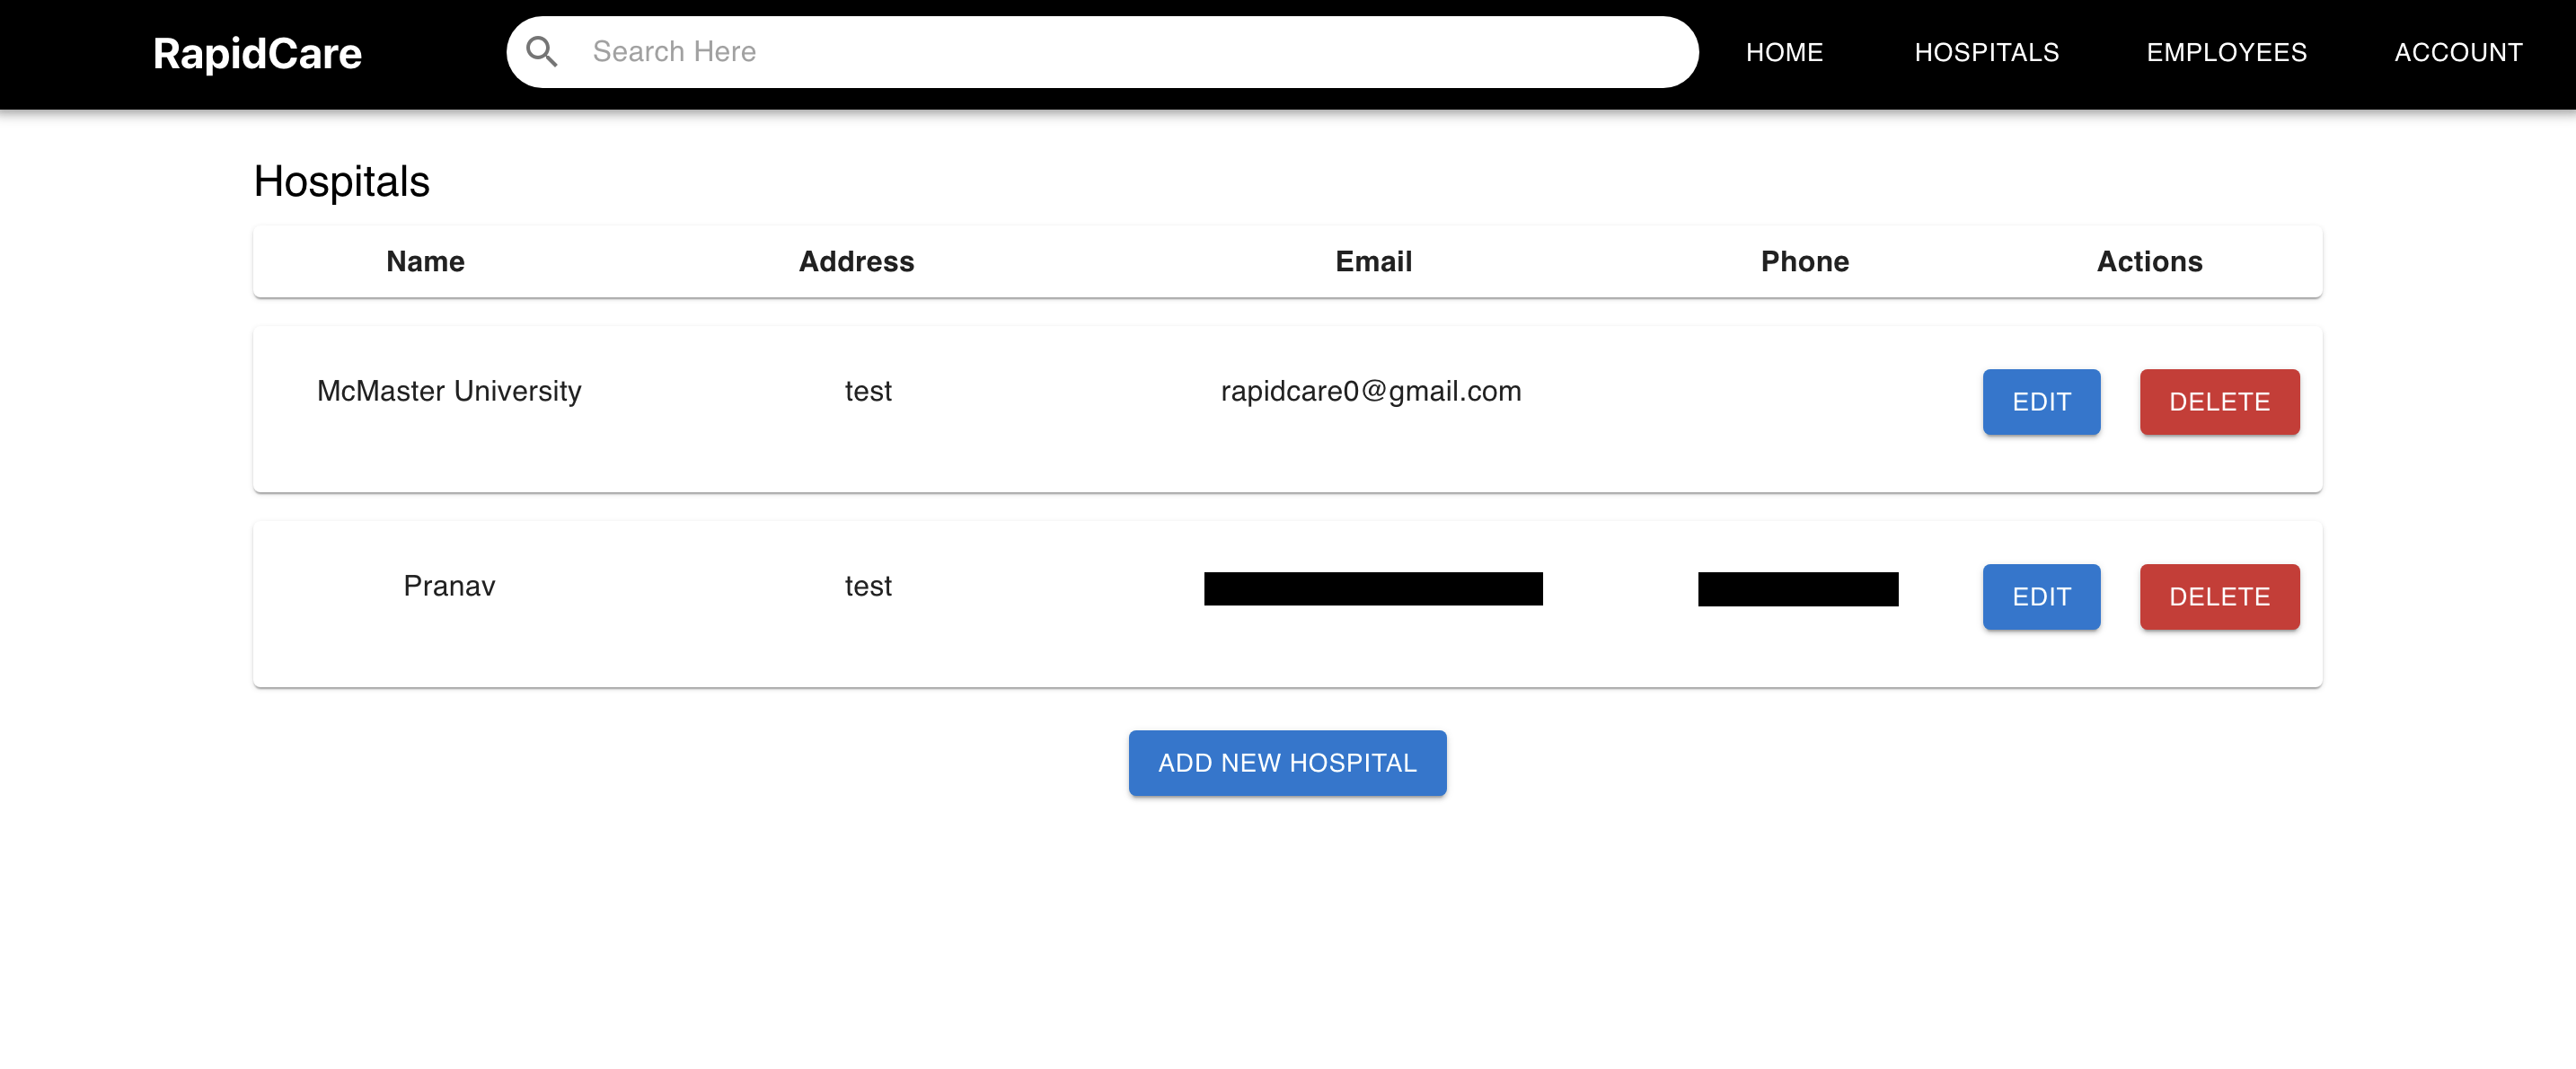
\includegraphics[width=0.9\textwidth]{hospital.png}
\caption{Hospital Management Interface}
\label{fig:Hospital Management Interface}
\end{figure}

\subsubsection{Adding a Hospital}
\begin{enumerate}
\item Log in with administrator credentials.
\item Navigate to "Hospitals".
\item Click "Add New Hospital".
\item Complete all required fields.
\item Click "Save" to add the hospital.
\end{enumerate}

\subsubsection{Updating Hospital Information}
\begin{enumerate}
\item Navigate to "Hospitals".
\item Select the hospital to update.
\item Click "Edit" button.
\item Edit the necessary fields.
\item Click "Save" to save changes.
\end{enumerate}

\subsubsection{Removing a Hospital}
\begin{enumerate}
\item Navigate to "Hospitals".
\item Select the hospital to remove.
\item Click "Delete" button.
\item Confirm the deletion when prompted.
\end{enumerate}

\subsection{Managing Healthcare Professionals}
For hospital administrators:

\begin{figure}[H]
\centering
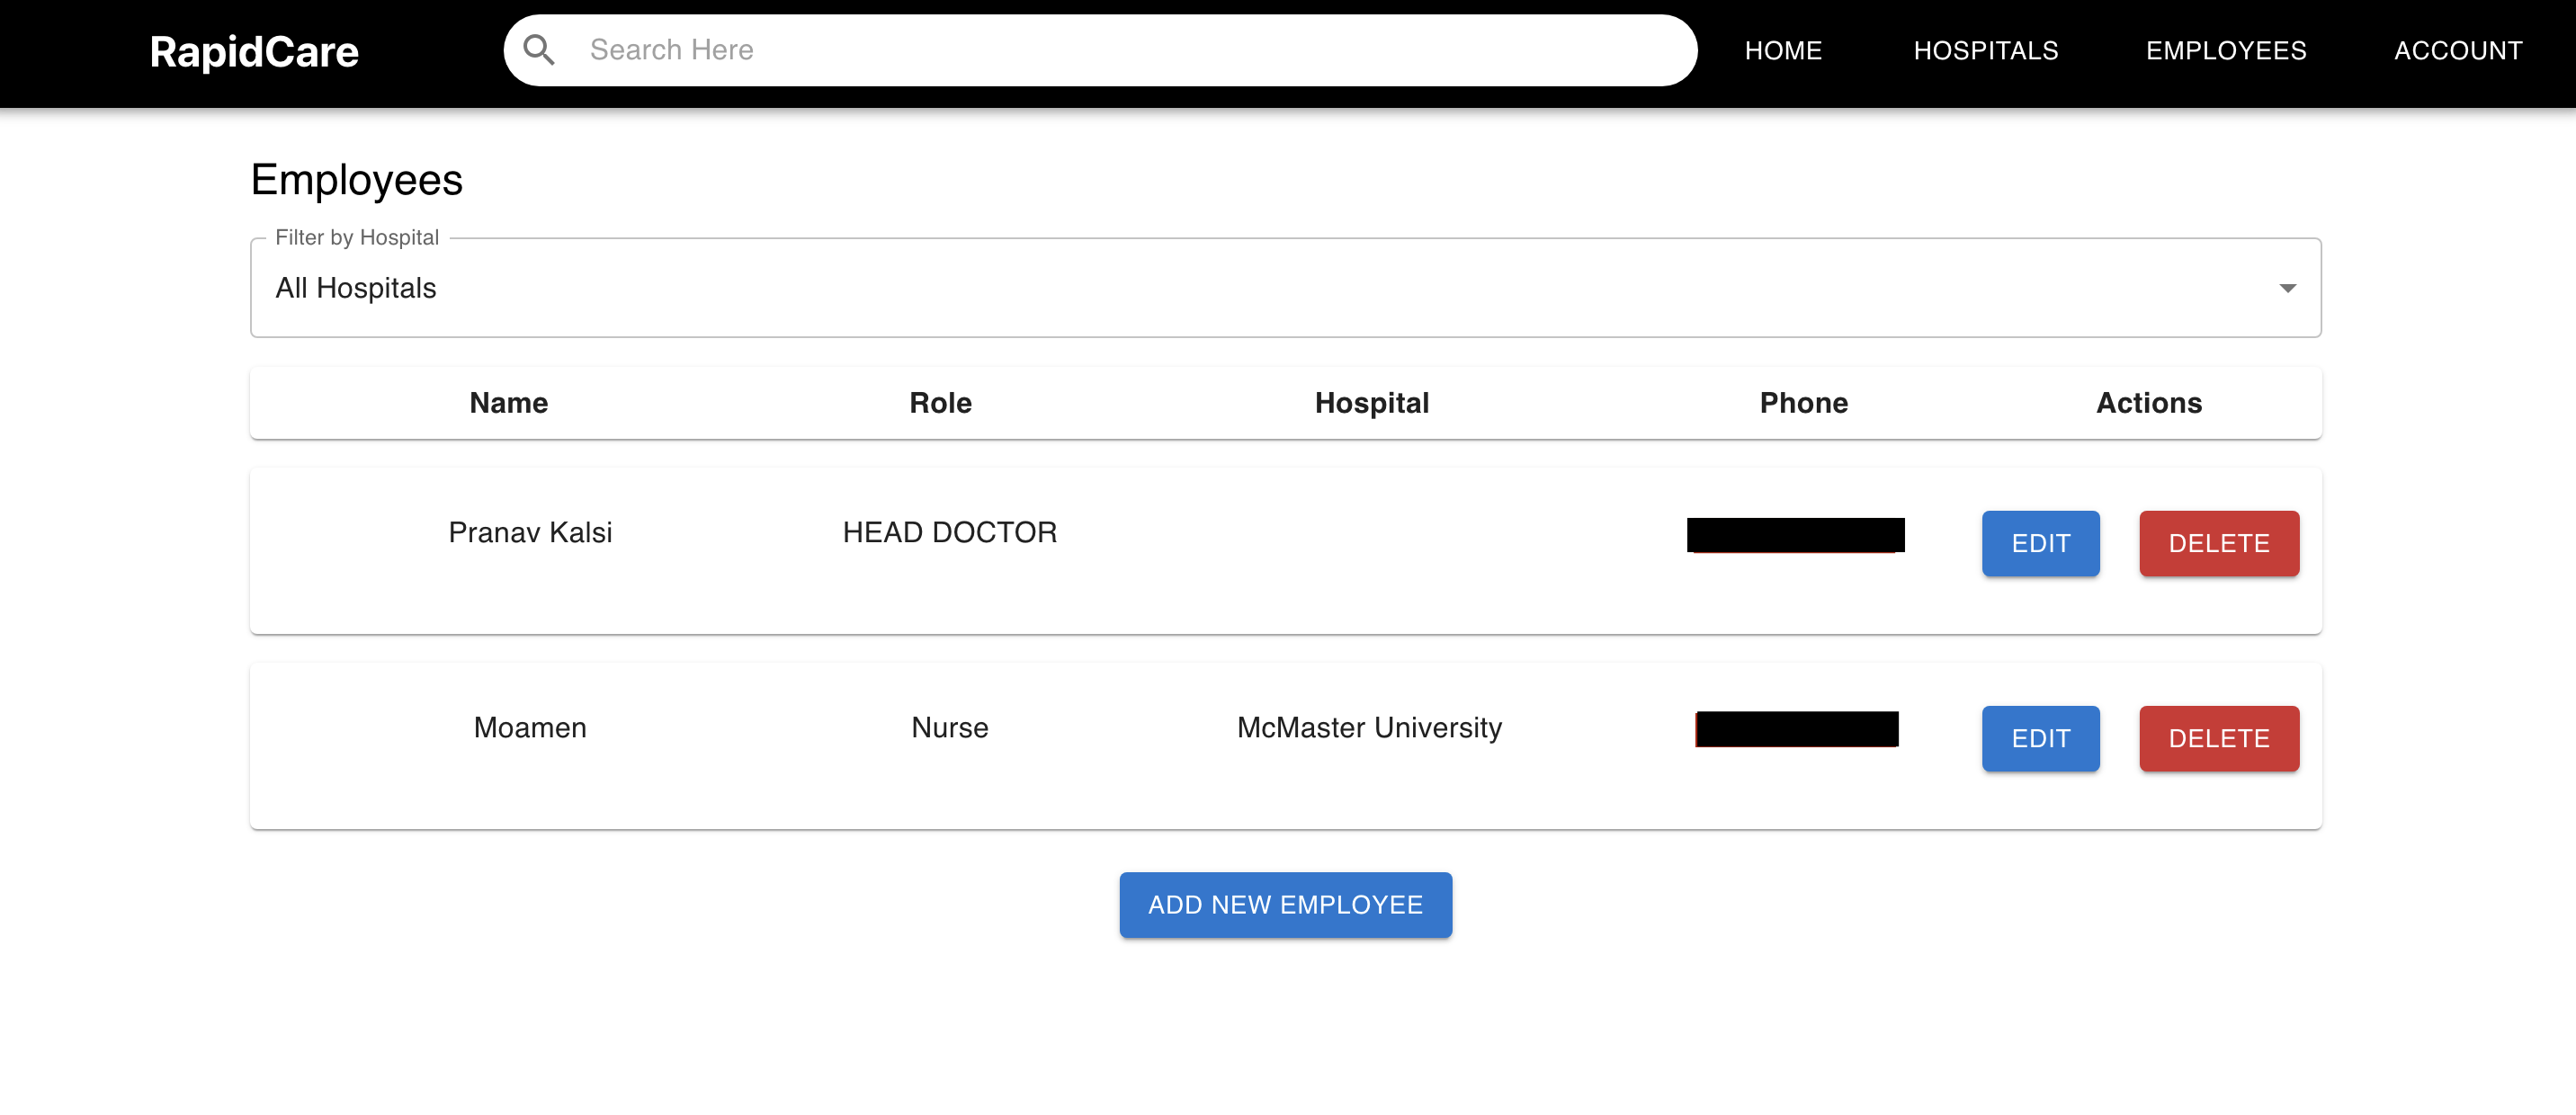
\includegraphics[width=0.9\textwidth]{employee.png}
\caption{Employee Management Interface}
\label{fig:Employee Management Interface}
\end{figure}

\subsubsection{Adding Healthcare Professionals}
\begin{enumerate}
\item Navigate to "Employees".
\item Click "Add New Employee".
\item Complete all required fields.
\item Set up initial credentials.
\item Click "Save" to add the professional.
\end{enumerate}

\subsubsection{Filtering Employees by Hospital}
\begin{enumerate}
    \item Navigate to "Employees".
    \item Click on the drop-down labeled "Filter by Hospital".
    \item Select a hospital from the list.
    \item The employee list will automatically update to display only employees associated with the selected hospital.
    \item To reset the view, select "All Hospitals" from the drop-down.
\end{enumerate}

\subsubsection{Updating Employee Information}
\begin{enumerate}
\item Navigate to "Employees".
\item Select the employee to modify.
\item Click "Edit" button.
\item Edit the necessary information.
\item Click "Save" to save changes.
\end{enumerate}

\subsubsection{Removing an Employee}
\begin{enumerate}
\item Navigate to "Employees".
\item Search for the employee.
\item Select the employee to remove.
\item Click "Delete" button.
\item Confirm the deletion when prompted.
\end{enumerate}

\subsection{Manage Administrator Network Account}
For hospital administrators:

\begin{figure}[H]
\centering
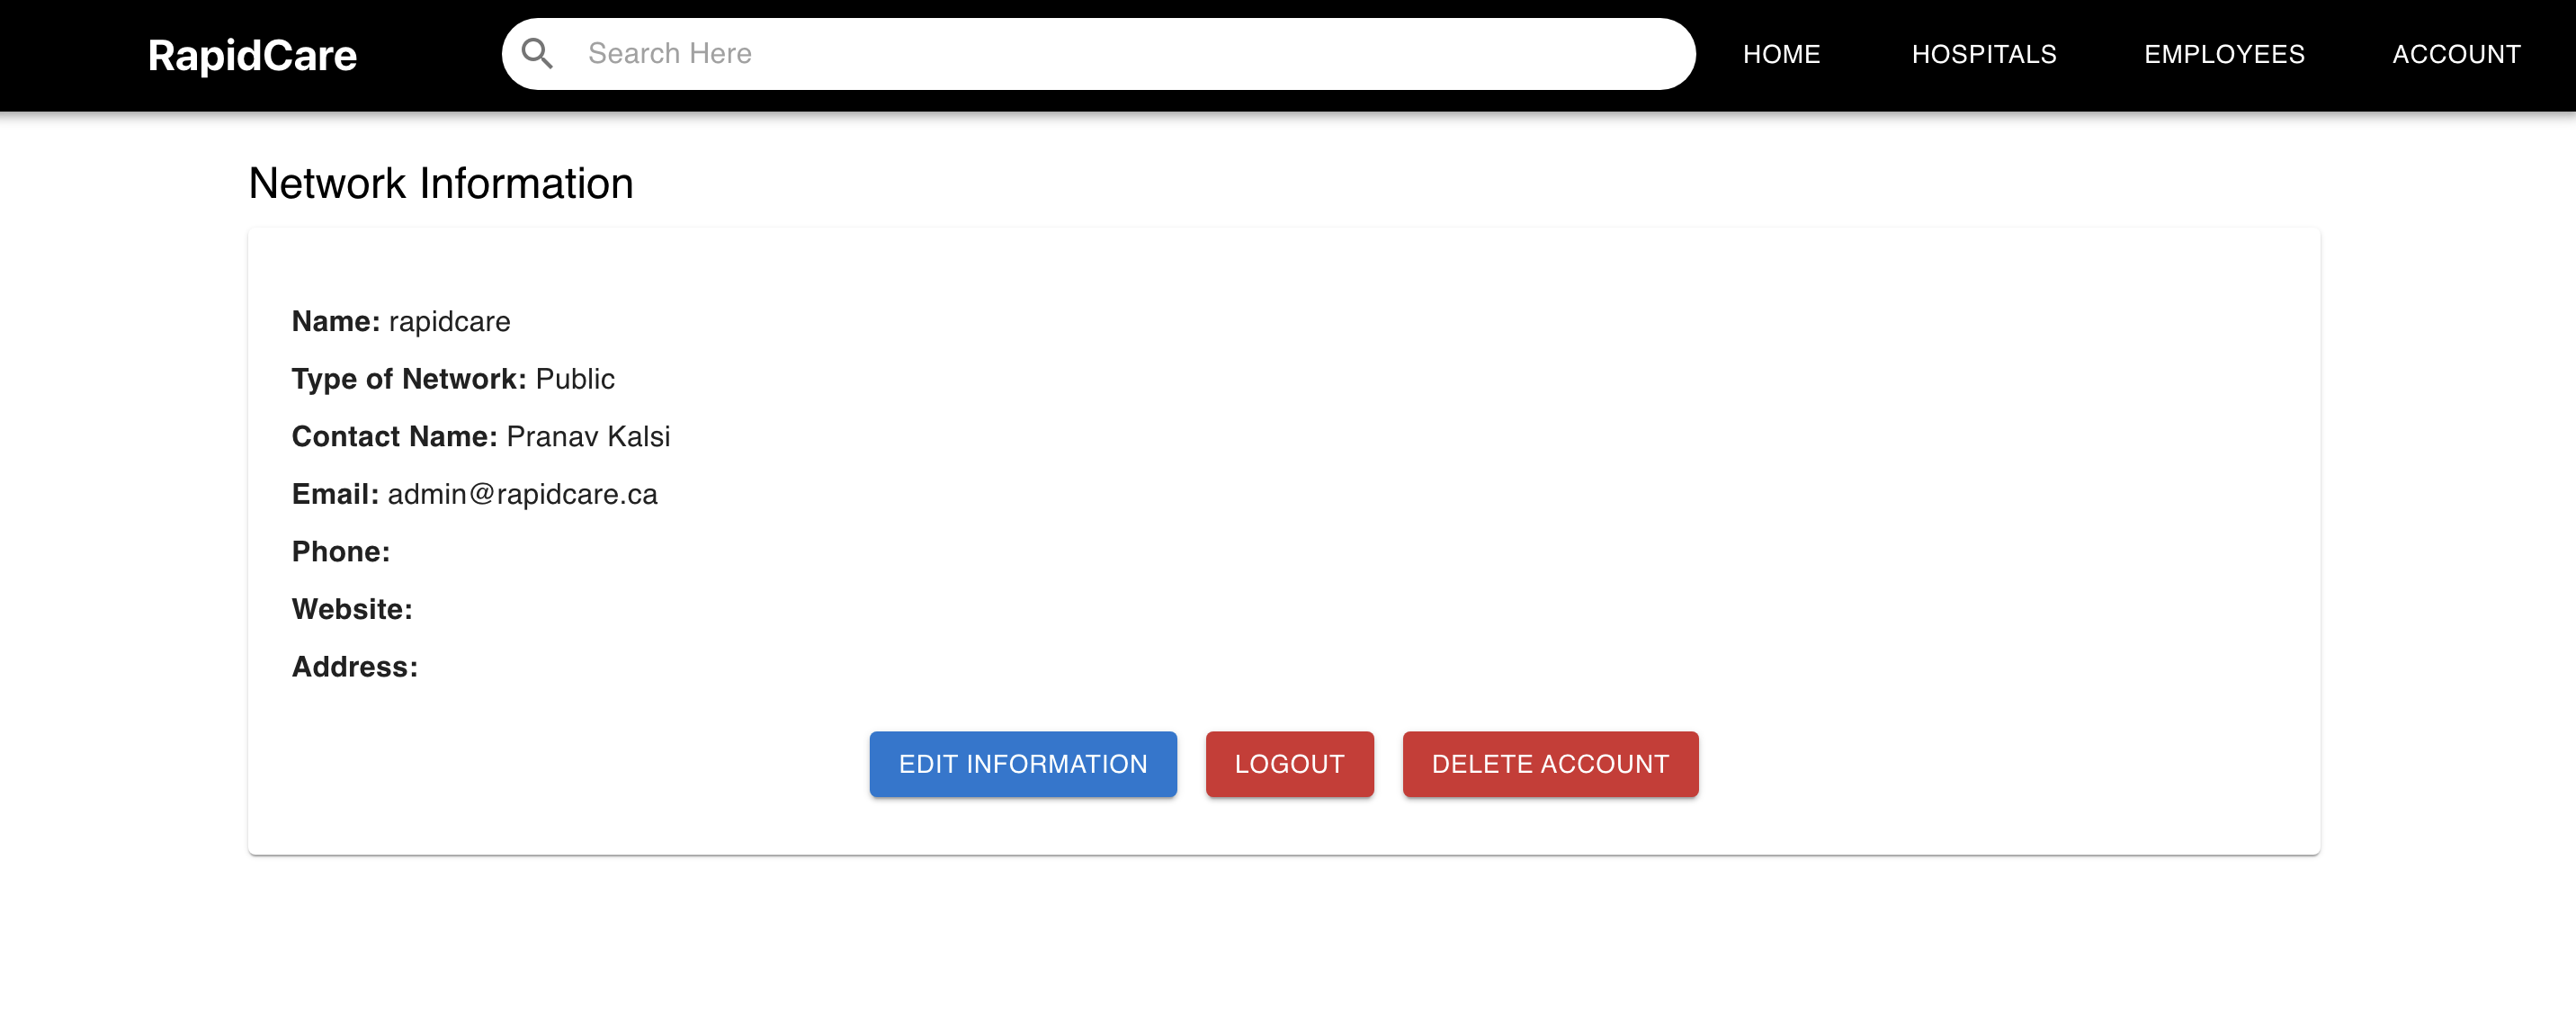
\includegraphics[width=0.9\textwidth]{account.png}
\caption{Adminstrator Account Management}
\label{fig:Adminstrator Account Management}
\end{figure}

\subsubsection{Editing Account Information}
\begin{enumerate}
    \item Navigate to "Account".
    \item Click the "Edit Information" button.
    \item Modify any necessary details.
    \item Click "Save" to apply changes.
\end{enumerate}

\subsubsection{Logging Out}
\begin{enumerate}
    \item Navigate to "Account".
    \item Click the "Logout" button.
\end{enumerate}

\subsubsection{Deleting Your Account}
\begin{enumerate}
    \item Navigate to "Account".
    \item Click the "Delete Account" button.
    \item Confirm the deletion when prompted. This action is irreversible and will permanently remove your account from the system.
\end{enumerate}

\subsection{Manage Healthcare Professional Account}
For healthcare professionals:

\begin{figure}[H]
\centering
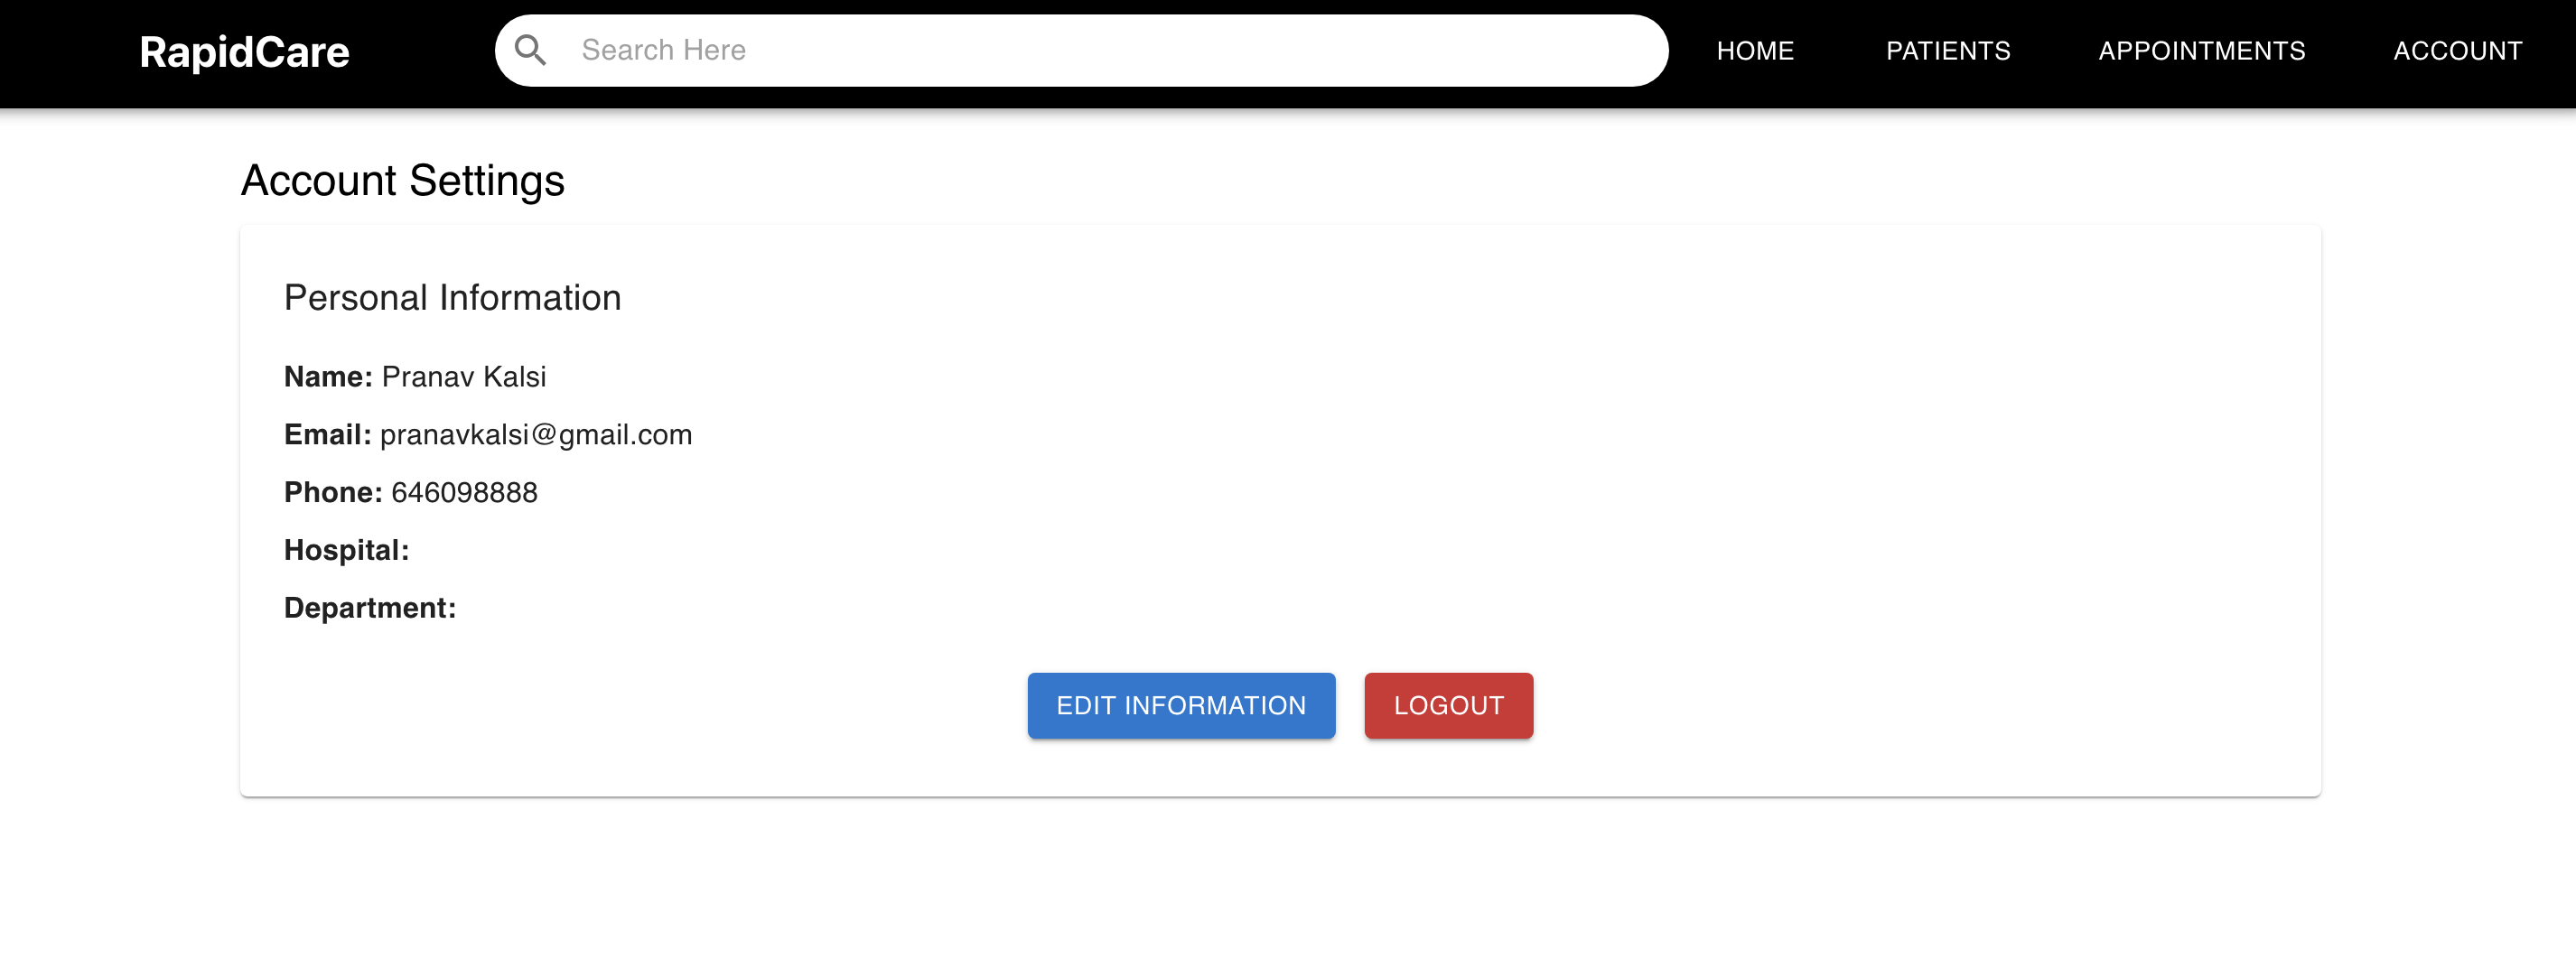
\includegraphics[width=0.9\textwidth]{employee_account.png}
\caption{Employee Account Management}
\label{fig:Employee Account Management}
\end{figure}

\subsubsection{Editing Account Information}
\begin{enumerate}
    \item Navigate to "Account".
    \item Click the "Edit Information" button.
    \item Modify any necessary account details.
    \item Click "Save" to apply changes.
\end{enumerate}

\subsubsection{Logging Out}
\begin{enumerate}
    \item Navigate to "Account".
    \item Click the "Logout" button.
\end{enumerate}


\section{Troubleshooting}
\subsection{Common Issues}
\begin{longtable}{p{0.3\textwidth}p{0.6\textwidth}}
\toprule
\textbf{Symptom} & \textbf{Solution} \\
\midrule
Login failures & Verify credentials, check caps lock. \\
Slow performance & Clear browser cache, check network. \\
Server crashes & Check logs, verify Firebase connection. \\
Transcription errors & Speak clearly, reduce background noise, review and edit transcriptions. \\
\bottomrule
\end{longtable}

\subsection{Error Messages}
\begin{itemize}
\item \textbf{ERR\_CONNECTION\_REFUSED}: Server may be down or unreachable.
\item \textbf{404 Not Found}: Verify URL or resource path.
\item \textbf{503 Service Unavailable}: Check server status.
\item \textbf{Authentication Failed}: Verify your credentials.
\end{itemize}

\section{Maintenance}
\subsection{Backup Procedures}
\begin{enumerate}
\item Run \texttt{backup create} command.
\item Store backup files securely in an off-site location.
\item Verify backup integrity regularly by performing test restorations.
\item Maintain a backup schedule to ensure data safety.
\end{enumerate}

\subsection{Updates}
\begin{itemize}
\item Check GitHub for new releases.
\item Follow upgrade instructions.
\item Test updates in staging environment first.
\item Schedule updates during off-peak hours to minimize disruption.
\end{itemize}

\section*{Acknowledgment}
The RapidCare development team thanks all users for their feedback and support in improving the system. Our goal is to reduce documentation overhead for healthcare professionals, enabling them to focus more on patient care and less on paperwork. Your continued feedback helps us enhance the system for better healthcare delivery.

\end{document}